%%%% Martin Rotter, Tomáš Kukučka, Jiří Zehnula - FJAA (zápisky z přednášek)
%%%%
%%%% kompilováno přes cslatex --> dvips --> ps2pdf
%%%%
%%%%%%%%%%%%%%%%%%%%%%%%%%%%%%%%%%%%%%%%%%%%%%%%%%%%%%%%%%%%%%%%%%%%%%%%%%%%%%%%%
%%%%%%%%%%%%%%%%%%%%%%%%%%%%%%%%%%%%%%%%%%%%%%%%%%%%%%%%%%%%%%%%%%%%%%%%%%%%%%%%%

\documentclass[10pt, a4paper, titlepage]{article}

\usepackage{czech}						% napsáno česky
\usepackage[utf8]{inputenc}				% napsáno v UTF-8
\usepackage[tables,figures]{upreport}	% UPOL styl
\usepackage{upstyles}
\usepackage{a4wide}
\usepackage{amsmath}
\usepackage{amssymb}
\usepackage{amsthm}
\usepackage{vaucanson-g}				% makro pro kreslení grafů a automatů
\usepackage{alltt}

\setlength{\parindent}{0pt}
\setlength{\parskip}{1ex plus 0.5ex minus 0.2ex}

\title{KMI/FJAA  -- Formální jazyky a automaty}
\author{M.~Rotter, T.~Kukučka, J.~Zehnula}
\date{\today}

\docinfo{M.~Rotter, T.~Kukučka, J.~Zehnula}{KMI/FJAA  -- Formální jazyky a automaty}

\newtheoremstyle{note}
{15pt}
{15pt}
{}
{}
{}
{:}
{.5em}
{}
\theoremstyle{note}
\newtheorem{veta}{\textbf{Věta}}
\newtheorem{definice}{\textbf{Definice}}
\newtheorem{dukaz}{\textbf{Důkaz}}
\newtheorem{priklad}{\textbf{Příklad}}
\newtheorem{poznamka}{\textbf{Poznámka}}
\newtheorem{dusledek}{\textbf{Důsledek}}

\abstract{Tento dokument je pouze přepisem zápisků a poznámek z přednášek předmětu KMI/FJAA. Přednášel \link{doc. Vilém Vychodil PhD}{http://vychodil.inf.upol.cz/}.}

\pagestyle{empty}
\makeindex

\begin{document}
\maketitle


\section{Historie}
Počátek úvah, jež byly později základem seriozního zkoumání formálních jazyků potažmo automatů se datuje do 30. let.
Průkopníkem této oblasti byl \link{Noam Chomsky}{http://cs.wikipedia.org/wiki/Noam_Chomsky}
\footnote{Jméno této osoby čti [\emph{čomski}] a zapamatuj si ke státnícím, že Chomsky byl \emph{nebezpečný levicový intelektuál}.}.

Jako příklad selhání autora programovacího jazyka si uveďme jazyk \textbf{Fortran}, jehož konstrukce byla po syntaktické stránce špatná,
což vedlo ke \textbf{gramatické nejednoznačnosti} tohoto jazyka.

\section{Kódová analýza}
\subsection{Lexikální analýza}
Dělení kódu na tokeny\footnote{Překládej jako \emph{část, díl nebo také fráze}.}, jež se zapisují například ve stylu
$\langle\text{ znak, identifikátor }\rangle$.
Příkladem je tedy i token $\langle =, assignment \rangle$ a jiné.

\subsection{Syntaktická analýza}
Syntaktická analýza vytváři stromovou závislost jednotlivých tokenů, jejíž reprezentace se nazývá \emph{syntaktický-derivační strom}.
V rámci této analýzy rozlišme:
\begin{enumerate}
\item
Teorii jazyků, jenž se zabýva stavbou jazyka (respektive jeho syntaxí) a poskytuje tzv. \textbf{generativní aparát}.
Dodejme, že gramatika řiká, v jakém tvaru může být zapsán validní program.

\item
Teorii automatů, jež poskytuje tzv. \textbf{analytický aparát}.
Dodejme, že automatem se rozumí de-facto jednoduchý algoritmus.
\end{enumerate}

\section{Základní pojmy}
\begin{itemize}
\item
\textbf{Symbol} (případně znak). Jedná se o syntaktický pojem (význam tedy nehraje roli), který představuje \emph{jméno} (analogicky k \emph{písmenu} z přirozeného jazyka).
Mezi symboly počítejme například \textbf{0, +, Š, while}.

\item
\textbf{Abeceda}. Abecedou rozumíme množinu (například množinu $X$) všech přípustných \emph{symbolů} (znaků), přičemž taková množina je neprázdná (tedy $|x|>0$) a konečná.
Konečnost množiny je omezení dané reprezentovatelností množiny v rámci počitačové techniky.
Abecedy značíme řeckými písmeny. Například $\Sigma, \Sigma^{'}, \Gamma, \ldots, \Omega$.
Například $\Sigma = \lbrace a, b, c \rbrace$.

\item
\textbf{Řetězec} (případně slovo). Jedná se o konečnou posloupnost symbolů (znaků) vybraných z nějaké dané abecedy.
Například $\langle a_{1}, a_{2}, \ldots, a_{n} \rangle \in \Sigma, n$ nazvěme \emph{délkou řetězce}.
Formálně definujme řetězec jakožto \emph{zobrazení}
$$
x : \lbrace a, b, c, d, \ldots, i, j, \ldots \rbrace \rightarrow \Sigma
$$
kde
$$
1 \rightarrow a, 2 \rightarrow b, 3 \rightarrow c
$$ a tak podobně.
Délku řetězce označme $|x|$.

\item
\textbf{Prázdný řetězec}. Jedná se o řetězec, pro který platí, že $|x| = 0$ a značíme jej $\varepsilon$, přičemž platí následujicí zápis:
$$
\varepsilon \subseteq \emptyset \rightarrow \Sigma
$$
Prázdný řetězec \textbf{není} symbolem, tedy $\varepsilon \notin \Sigma$.
\end{itemize}

\begin{veta}
Nad $k$-prvkovou abecedou je právě $k^{n}$ řetězců délky $n$.
\end{veta}


\begin{poznamka}
Uveďme si rovněž značení pro dva důležíté pojmy:

\begin{itemize}
\item
$\Sigma^{*}$ označuje množinu všech řetězců nad abecedou$\Sigma$.

\item
$\Sigma^{+}$ označuje množinu všech řetězců nad abecedou$\Sigma$ vyjma $\varepsilon$.
\end{itemize}
\end{poznamka}

\section{Operace s řetězci}
\begin{itemize}
\item
\textbf{Zřetězení} (konkatenace). Jde v podstatě o spojení\footnote{Pro milovníky jazyka Scheme můžeme tuto operaci přirovnat k proceduře \emph{append}}
dvou řetězců v daném pořadí do jednoho řetězce.

\begin{priklad}
Mějme dva řetězce $a$, $b$:
$$
a_{1}\ldots a_{n} \text{ a } b_{1}\ldots b_{m}
$$
Pak jejich zřetězení má tvar:
$$
a_{1}\ldots a_{n}b_{1}\ldots b_{m}
$$
Identifikátorem\footnote{Identifikátor zřetězení se velmi čast v zápisech zřetězení vynechává.} operace
zřetězení je $\circ$, například $x\circ y$ je zřetězením řetězců $x$ a $y$.
Formálně takto:
\begin{gather*}
x : \lbrace 1,\ldots, n \rbrace \rightarrow \Sigma \\
y : \lbrace 1,\ldots, m \rbrace \rightarrow \Sigma \\
x \circ y : \lbrace 1,\ldots, nm \rbrace \rightarrow \Sigma
\end{gather*}
\end{priklad}

\begin{poznamka}
Algebraicky je tatáž operace zapsána jako $\langle \Sigma^{*}, \circ, \varepsilon \rangle$.
\end{poznamka}

\item
\textbf{Rovnost řetězců}
Pro prohlášení dvou řetězců za sobě rovné v žádaném smyslu je třeba splnit obecně dvě následující podmínky:
\begin{enumerate}
\item
Oba řetězce mají stejnou délku, tedy $|x| = |y|$.

\item
Bude-li délka označena jako $n$, pak musí platit, že $\forall i | i \in \lbrace 1, \ldots, n \rbrace, x(i) = y(i)$.
Tedy každé dva k sobě náležící symboly z daných řetězců jsou si rovny.
\end{enumerate}
Uvažujeme-li rovnost řetězců, pak je záhodno uvažovat následující pojmy:
\begin{itemize}
\item
\textbf{Prefix} řetězce. Označme jej $Pfx(x) = \lbrace y | \exists z \text{ tak, že } yz = x \rbrace$.

\item
\textbf{Infix} řetězce. Označme jej $Ifx(x) = \lbrace y | \exists z_{1}, z_{2} \text{ tak, že } z_{1}yz_{2} = x \rbrace$.

\item
\textbf{Sufix} řetězce. Označme jej $Sfx(x) = \lbrace y | \exists z \text{ tak, že } zy = x \rbrace$.
\end{itemize}

\begin{veta}
\begin{gather*}
xy = xz \: \Longrightarrow \: y = z \\
yx = zx \: \Longrightarrow \: y = z
\end{gather*}
Algebraicky je operace zapsána jako $\langle \Sigma^{*}, \cdot, \varepsilon \rangle$.
\end{veta}

\begin{veta}
Vyslovme předpoklad, že platí $xy = uv$. Pak platí právě jedno z těchto tvrzení:
\begin{gather*}
x = u, y = v \\
|x| > |u| \text{ a } \exists w| w \neq \varepsilon, \text{ tak že } x = uw \text{ a } v = wy \\
|x| < |u| \text{ a } \exists w| w \neq \varepsilon, \text{ tak že } u = xw \text{ a } y = wv
\end{gather*}
\end{veta}

\item
\textbf{N-tá mocnina} řetězce.
$$
x^{n} = \left\lbrace
\begin{array}{l l}
x & \text{pro } n=1 \\
xx^{n-1} & \text{v ostatních případech} \\
\end{array}
\right\rbrace
$$
respektive
$$ x^{n} = \left\lbrace
\begin{array}{l l}
\varepsilon & \text{pro } n=0 \\
xx^{n-1} & \text{v ostatních případech} \\
\end{array}
\right\rbrace
$$
\begin{poznamka}
Mějme na paměti, že operace mocnění má vyšší prioritu než-li operace konkatenace (zřetězení).
\end{poznamka}

\begin{veta}
Mějme $u \text{ a } v \in \Sigma^{*}$, pak platí $uv = vu$ (komutativita), právě
tehdy, když $\exists z| z \in \Sigma^{*} \text{ a nezáporná celá čísla } p, q \text{ tak, že } u = z^{p} \text{ a } v=z^{a}$.
\end{veta}

Předpokládejme, že po $p, z, q$ máme $u = z^{p}, v = z^{q}$. Pak obecně platí následující zápis:
$$
uv = z^{p}z^{q} = z^{p+q} = z^{p} z^{q} = vu
$$

Předpokládejme, že $uv = vu$. Indukcí přes $|uv|$ předpokládáme, že tvrzení platí pro libovolné dva řetězce, jejichž délka zřetězení je menší
než-li $|uv|$. Mohou nastat tyto případy:
\begin{enumerate}
\item
$|u| = |v|, \text{ pak } u = v, \text{ pak } z = u, p = q = 1$

\item
$|u| < |v|$
\end{enumerate}

Berme v potaz také následující zápis doplněný obrázkem: \ref{obr-1}

\begin{gather*}
uv = v \\
wu = v \\
uw = wu \\
|uw| < |uv|, \text{ tedy } \exists z, p, q  \text{ tak, že } u = z^{p}, w = z^{q}, v = z^{p+q}
\end{gather*}

\begin{figure}[ht]
\centering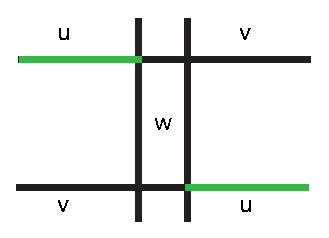
\includegraphics[width=5cm]{dukaz-1.eps}
\caption{Grafická pomůcka ke komutativitě zřetězení řetězců.}\label{obr-1}
\end{figure}
\end{itemize}

\section{Formální jazyk}
Zaveďme si pojem \emph{formální jazyk nad množinou všech řetězců} $\Sigma^{*}$. Označme tento jazyk jako $L$. Pak platí tato tvrzení:
\begin{eqnarray*}
L &\subseteq& \Sigma^{*} \text{ (každá podmnožina abecedy je jazykem)} \\
L &=& \emptyset \text{ (prázdný jazyk)} \\
L &=& \lbrace \varepsilon \rbrace \text{ (jazyk s prázdným řetězcem)} \\
L &=& jazyk C++ \text{ (jazyk C++)} \\
&\vdots&
\end{eqnarray*}
\textbf{Pozor, obecně platí že prázdný jazyk $\neq$ jazyk s prázdným řetězcem.}
	
\section{Lexikografické uspořádání}
Předpokládejme uspořádání na množině $\Sigma^{*}$.
Nazvěme toto uspořádání \emph{striktním totálním}. Pak toto uspořádání například pro $\Sigma = \lbrace a_{1}, \ldots, a_{n} \rbrace$
je $a_{1} < a_{2} < a_{3} < \ldots < a_{n}$.

Totální striktní uspořádání označme $<_{l}$.

Položme $x <_{l} y$ pro $x,y \in \Sigma^{*}$. To ale platí pokud platí alespoň jedno z následujících dvou tvrzení:
\begin{enumerate}
\item
$|x| < |y|$

\item
$|x| < |y| \text{ a } \exists i \text{ tak, že } x(i) < y(i) \text{ a zároveň } x(j) < y(j) \text{ pro } \forall j |j < i$
\end{enumerate}

\begin{priklad}
$\Sigma = \lbrace 0, 1 \rbrace$. Triviálně tedy $0 < 1$.
Následně striktně $\varepsilon <_{l} 0 <_{l} 1 <_{l} 00 <_{l} 01 <_{l} 10 <_{l} 11$.
\end{priklad}

\begin{veta} \label{veta-1}
Striktní totální uspořádání je asymetrické a tranzitivní. A pro $x \neq y$ platí buď $x <_{l} y$ nebo $y <_{l} x$.
\end{veta}

\begin{dusledek}
Důsledkem věty \ref{veta-1} je tvrzení, že množina $\Sigma^{*}$ je spočetně nekonečná. Dodejme, že jazyk je (obvykle) spočetná množina.
\end{dusledek}

\section{Operace nad jazyky}
\nextoutline{Mnozinové}

\subsection{Množinové}
Množinové operace nad jazyky jsou prakticky totožné operacím na kterýchkoliv jiných množinách. Můžeme tedy použít množinový průnik, sjednocení, komplement (doplněk) nebo rozdíl.

\subsection{Ostatní}
\begin{itemize}
\item
\textbf{Zřetězení} (produkt) množin. Vyjádřeme produkt takto:
$$
L_{1}L_{2} = \lbrace xy | x \in L_{1}, y \in L_{2} \rbrace
$$
Produkt množin není obecně komutativní, ale je asociativní, přičemž prázdná množina tuto operaci anihiluje.
Uveďme si rovněž monoid $\langle 2^{\Sigma^{*}}, \circ, \lbrace \varepsilon \rbrace \rangle$.

\item
\textbf{Mocnina} jazyka. Mocninu vyjádříme takto:
$$
L^{n} = \left\lbrace
\begin{array}{l l}
\lbrace \varepsilon \rbrace & \text{ pro } n = 0 \\
LL^{n-1} & \text{ pro } n > 1 \\
\end{array}
\right\rbrace
$$

\item
\textbf{Kleeneho\footnote{\link{Stephen Cole Kleene}{http://en.wikipedia.org/wiki/Stephen_Cole_Kleene} je známý matematik, jenž se významně podílel na položení základů teoretických počítačových věd.}} uzávěr neboli \textbf{iterace}. Tento uzávěr vyjádříme takto:
$$
L^{*} = \bigcup_{i = 0}^{\infty} L^{i}
$$

\item
\textbf{Pozitivní} uzávěr neboli pozitivní iterace. Tento uzávěr vyjádříme takto:
$$
L^{+} = \bigcup_{i = 1}^{\infty} L^{i}
$$
Všimněte si podobností mezi těmito dvěma uzávěry. Pozitivní uzávěr vynechává prázdný řetezec.

\end{itemize}

\section{Gramatiky}
Jak víme, tak jazyky mohou být \emph{nekonečné} ve smyslu, že obsahují nekonečný počet slov.
Nabízí se tedy otázka, jak tyto jazyky rozumně popsat, jak je reprezentovat resp. jak vytvořit \emph{konečnou}
sadu pravidel, jejichž aplikace by vedla k opětovné generaci původního jazyka.

\nextoutline{Prepisovací generovací pravidla}
\subsection{Přepisovací generovací pravidla}
Pravidlem rozumíme zpravidla každou takto definovanou dvojici.
$$
\langle x,y \rangle \in \Sigma^{*} \times \Sigma^{*}
$$
Pak neformálně tvrdíme, že $x$ \emph{se přepisuje} na $y$.
Nutno dodat, že předchozí zápis lze zapsat i například takto.
$$
x \rightarrow y\text{, kde symbol } \rightarrow \notin \Sigma \text{ můžeme prohlásit za tzv. metasymbol.}
$$
\subsubsection{Vlastnosti pravidel}
\begin{itemize}
\item \emph{Nezkracující} pravidlo je pravidlo, o kterém platí, že $|x| \leq |y|$. Tedy aplikaci tohoto pravidla na vstupní řetězec určitě nevznikne řetězec kratší, než-li jeho předloha.

\item $\varepsilon$ - pravidlo je pravidlo tvaru $x \rightarrow \varepsilon$.
\end{itemize}

\nextoutline{Priklady pravidel}
\subsubsection{Příklady pravidel}
\begin{priklad}
Mějme zadání abecedy $\Sigma = \lbrace a,b,c \rbrace$. Pravidla s využítím této abecedy by mohla být například tato.
\begin{eqnarray*}
aa &\rightarrow& bc \\
bb &\rightarrow& y \\
c &\rightarrow& \varepsilon
\end{eqnarray*}
\end{priklad}

\begin{priklad}
Mějme další zadání abecedy $\Sigma = \lbrace expr, +, \times \rbrace$. Pravidla s využítím této abecedy by mohla být například tato.
\begin{eqnarray*}
\textit{expr} &\rightarrow& \textit{expr} + \textit{expr} \\
\textit{expr} &\rightarrow& \textit{expr} \times \textit{expr}
\end{eqnarray*}
\end{priklad}

\nextoutline{Prime odvozovani rezezcu pomoci pravidel}
\subsubsection{Přímé odvozování řetězců pomocí pravidel}
Uvažujme odvozovací pravidlo $ x \rightarrow y \text{ nad abecedou } \Sigma$, pak řekneme, že řetězec \emph{v} \textbf{je přímo odvozen}
z řetězce \emph{u} pomocí pravidla $ x \rightarrow y $, pokud $\exists p, q \in \Sigma^{*}$ tak, že
\begin{gather*}
u = p x q \\
v = p y q
\end{gather*}

Značení předchozí operace je následující:
$$
u \Rightarrow_{x \rightarrow y} v
$$
Slovně bychom tento zápis vystihli jako \uv{přímý přepis dle pravidla $x \rightarrow y$.}

Řetězec $v$ vznikne přímým přepisem z $u$ pomocí pravidel $P \subseteq  \Sigma^{*} \times \Sigma^{*}$, pokud
$\exists \pi \in P \text{ tak, že } u \Rightarrow_{\pi} v$.

Značme $u \Rightarrow_{P} v$. $P$ je množinou užitých pravidel. $P$ i $\Rightarrow_{p}$ jsou binární relace na $\Sigma^{*}$ a
$P \subseteq  \Rightarrow_{p}$, tedy \uv{P je podmnožinou šipky p.} Platí, že $x \rightarrow y \in P$ a $x \Rightarrow_{x \rightarrow y} y$.

\begin{priklad}
Mějme abecedu $\Sigma = \lbrace a, b, c \rbrace$ a soubor pravidel $P = \lbrace aa \rightarrow bc, a \rightarrow cab, bb \rightarrow \varepsilon \rbrace$\label{priklad-1}.
Pak by odvození v jednom kroku mohla vypadat například takto:
\begin{gather*}
baaa \rightarrow bbca \\
bac \rightarrow bcabc
\end{gather*}
\end{priklad}

\begin{definice}
Definujme pojem \textbf{derivace}. Jedná se o posloupnost řetězců ve tvaru:
$$
x_{0}, \ldots, x_{k},\text{ kde } k \geq 0\text{ a kde } \lbrace x_{0}, \ldots, x_{k} \rbrace \in \Sigma^{*}
$$
se nazývá \textbf{P-derivace délky k}, pokud $x_{i-1} \Rightarrow_{p} x_{i}, \forall 1 \leq i \leq k $.
Symbolicky totéž $x_{0} \Rightarrow_{p} x_{1} \Rightarrow_{p} \ldots \Rightarrow_{p} x_{k}$. Počet odvození tedy značí \emph{délku} derivace.
\end{definice}

Pokud pro $u, v \in \Sigma^{*} \exists \text{ P-derivace } u = x_{0} \ldots x_{k} = v$, pak říkáme, že $v$ je odvozeno z $u$ pomocí pravidel z $P$, což značíme
například $u \Rightarrow_{P}^{*} v$, tímto je pochopitelně myšleno odvození ve více krocích. Platí, že $P \subseteq \Rightarrow_{P} \subseteq \Rightarrow_{P}^{+}$.

\begin{priklad}
Mějme abecedu $\Sigma = \lbrace a, \ldots, z \rbrace$ a pravidla stejná jako v příkladu \ref{priklad-1}.
Nyní odvozujeme například takto:
$$
b\underline{aa}a, \underline{bb}ca, c\underline{a}, c\underline{cab}
$$
\end{priklad}

\subsection{Formální gramatiky}
Mějme následující entity:
\begin{itemize}
\item $\Sigma$ - abeceda terminálních symbolů (tyto symboly tvoří řetězce daného jazyka).
\item $N$ - abeceda neterminálních symbolů (tyto symboly se užívají k řízení průběhu odvozování).
\end{itemize}

Dodejme, že obě množiny by měly být neprázdné a konečné.

\begin{definice}
Odvozovací pravidlo $x \rightarrow y$ se nazývá \emph{generativní}, pokud \emph{x} obsahuje alespoň jeden neterminální symbol.
\end{definice}

\begin{definice}
Mějme strukturu $G = \langle N, \Sigma, R, S \rangle$, kde \emph{N} je abecedou neterminálních symbolů, $\Sigma$ je abecedou terminálních symbolů,
\emph{P} je množinou odvozovacích pravidel a $S \in N$\hyplabel{terminal} je tzv. \emph{počátečním} resp. \emph{startovním} neterminálem. Pak tuto čtveřici nazveme \textbf{gramatikou}.
\end{definice}

\begin{poznamka}
Pokud chceme vyjádřit, že z jednoho symbolu odvozujeme několik možných alternativ, tak to zapíšeme místo klasického dlouhé zápisu
$y \rightarrow x_{1}, y \rightarrow x_{2}, \ldots$ pomocí zkrácené notace např. $y \rightarrow x_{1}|x_{2}|\ldots$
\end{poznamka}

\begin{priklad}
Gramatikou může vypadat třeba takto:
\begin{eqnarray*}
N &=& \lbrace \varepsilon, S, D, I \rbrace \\
\Sigma &=& \lbrace 0, \ldots, 9, +, - \rbrace \\
P &=& \lbrace S \rightarrow -I|+I|I, I \rightarrow DI|D, D \rightarrow 0|1|\ldots |9 \rbrace \\
G &=& \langle N, \Sigma, P, S \rangle
\end{eqnarray*}
\end{priklad}

\begin{priklad}
Nebo tato.
\begin{eqnarray*}\label{priklad-2}
N &=& \lbrace S, X, Y \rbrace \\
\Sigma &=& \lbrace a, b, c \rbrace \\
P &=& \lbrace S \rightarrow XcYcX, X \rightarrow aX, X \rightarrow bX, X \rightarrow cX, X \rightarrow \varepsilon,
y \rightarrow abY, Y \rightarrow ab \rbrace \\
G &=& \langle N, \Sigma, P, S \rangle
\end{eqnarray*}
\end{priklad}

\begin{definice}
Každý řetězec $x \in (N \cup\Sigma)^{*}$, pro který platí $S \rightarrow^{*} x$, je \textbf{větná forma} gramatiky $G = \langle N, \Sigma, P, S \rangle$.
Větná forma se nazývá \textbf{větou}, pokud $x \in \Sigma^{*}$.
\end{definice}

\begin{definice}
Jazyk generovaný gramatikou definujme jako:
$$
L(G) = \lbrace x \in \Sigma^{*} | S \Rightarrow_{G}^{*} x \rbrace
$$
Vidíme tedy, že takový jazyk obsahuje \emph{věty}, které lze odvodit ze startovacího neterminálu pomocí pravidel této gramatiky.
\end{definice}

\begin{priklad}
Tento příklad čerpá gramatiku z příkladu \ref{priklad-2}.
\begin{eqnarray*}
S &\Rightarrow_{G}^{*}& abbccYcX \\
S &\Rightarrow_{G}^{*}& Xcababababc \\
S &\Rightarrow_{G}^{*}& cYcbaX \\
S &\Rightarrow_{G}^{*}& abbccabca \\
S &\Rightarrow_{G}^{*}& cabababc
\end{eqnarray*}
\end{priklad}

\begin{definice}
Gramatiky $G_{1}$ a $G_{2}$ jsou \textbf{ekvivalentní}, pokud generují stejný jazyk.
\end{definice}

\subsection{Hierarchie gramatik}
\begin{itemize}
\item
\textbf{Gramatiky typu 0} -- jedná se o gramatiky bez omezení.

\item
\textbf{Gramatiky typu 1\label{gram-1}} -- jedná se o tzv. \emph{kontextové} nebo \emph{kontextově závislé} gramatiky.
Ty splňují následující omezení na tvar pravidel. Pro každé pravidlo gramatik tohoto typu platí, že:
\begin{enumerate}
\item
Buď je (pravidlo) ve tvaru $pAq \rightarrow p \times q, \text{ kde } p, q \in (\Sigma \cup N)^{*}, A \in N, x \in (\Sigma \cup N)^{*}$, kde \emph{p} a \emph{q}
se nazývají levým resp. pravým \textbf{kontextem}.

\item
Nebo je (pravidlo) ve tvaru $S \rightarrow \varepsilon$, kde $S$ je \emphref{startovní terminál}{terminal} gramatiky, ale pouze
za předpokladu, že $S$ se nevyskytuje na pravé straně žádného pravidla.
\end{enumerate}

\item
\textbf{Gramatiky typu 2} -- jedná se o tzv. \emph{bezkontextové} gramatiky, jenž obsahují pravidla ve tvaru:
$$
A \rightarrow x, \text{ kde } A \in N, x \in (\Sigma \cup N)^{*}
$$
Na levých stranách pravidel tedy očekáváme pouze neterminální symbol.

\begin{priklad}
Mějme tuto gramatiku:
\begin{eqnarray*}
G &=& \langle N, \Sigma, P, S \rangle \\
N &=& \lbrace A, S \rbrace \\
\Sigma &=& \lbrace 0, 1 \rbrace \\
P &=& \lbrace S \rightarrow 0A, A \rightarrow \varepsilon \rbrace
\end{eqnarray*}
\end{priklad}

\item
\textbf{Gramatiky typu 3\label{gram-3}} -- jedná se o tzv. \emph{regulární} resp. \emph{pravolineární} gramatiky, které obsahují pravidla ve třech následujících tvarech:

\begin{enumerate}
\item
$A \rightarrow bB, \text{ kde } A,B \in N, b \in \Sigma$

\item
$A \rightarrow a$

\item
$S \rightarrow \varepsilon$
\end{enumerate}

\end{itemize}

\begin{poznamka}
Každý konečný jazyk je regulární.
\end{poznamka}

\begin{dukaz}
Mějme jazyk $L = \lbrace x_{1},\ldots, x_{n} \rbrace$. Abychom tento jazyk prohlásili za regulární, tak je třeba najít regulární gramatiku,
která tento jazyk generuje.

Mějme tedy nějaké dané $\Sigma \text{ a } S$ a zvolme \emph{N}. Následně platí $\forall x_{i} \in L$ je dvojího typu:

\begin{enumerate}
\item
$x_{i} = \varepsilon \text{ a následně } S \rightarrow \varepsilon$

\item
$x_{i} = a_{1}\ldots a_{k} \text{ a následně } S \rightarrow a_{i1}A^{'}, A^{'} \rightarrow a_{i2}A^{''},\ldots\ldots, A^{k-1} \rightarrow a_{ik}A^{k}$
\end{enumerate}
\end{dukaz}

\begin{figure}[ht]
\centering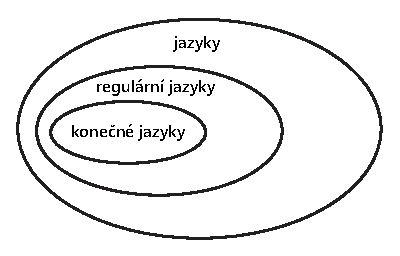
\includegraphics[width=8cm]{vajicko-1.eps}
\caption{Vychodilovo \uv{vajíčko.}}\label{obr-2}
\end{figure}

\vspace{30px}

\begin{priklad}
\begin{eqnarray*}
N &=& \lbrace S \rbrace \\
\Sigma &=& \lbrace a, b \rbrace \\
P &=& \lbrace S \rightarrow aSb | \varepsilon \rbrace \\
L(G) &=& \lbrace a^{n}b^{n} | n \leq 0 \rbrace
\end{eqnarray*}
Máme tedy \emph{bezkontextový} jazyk.
\end{priklad}

\begin{priklad}
\begin{eqnarray*}
N &=& \lbrace S \rbrace \\
\Sigma &=& \lbrace a, b \rbrace \\
P &=& \lbrace S \rightarrow SS|aSb|bSa| \varepsilon \rbrace
\end{eqnarray*}
$L(G)$ je \emph{bezkontextový} jazyk.
\end{priklad}

\begin{priklad}
\begin{eqnarray*}
N &=& \lbrace S, V \rbrace \\
\Sigma &=& \lbrace p,),(, \Rightarrow, ! \rbrace \\
P &=& \lbrace S \rightarrow V|(S \Rightarrow S)|!S, V \Rightarrow pV|p \rbrace
\end{eqnarray*}
$L(G)$ je jazyk všech výrokových formulí.
\end{priklad}

%%%%%%%%%%%%%%%%%%%%%%%%%%%%%%%%%%%%%%
%%%%%%%%%%%%%%%%%%% 3. a 4. přednáška - Tom


\subsection{Gramatika nezkracující}
Gramatika G se nazývá nezkracující, pokud má pouze nezkracující pravidla a může mít pravidlo ve tvaru $S \rightarrow \varepsilon$, přičemž $S$ se nenachází na žádné z pravých stran.

\begin{priklad}
\begin{eqnarray*}
N &=& \lbrace S, A, B, C\rbrace \\
\Sigma &=& \lbrace a, b, c\rbrace \\
P &=& \lbrace S \rightarrow \varepsilon |abc|Ac, A \rightarrow aBcb, Bcb \rightarrow bBc, Bcc \rightarrow Ccc, bc \rightarrow Cb, aC \rightarrow aab|aA \rbrace
\end{eqnarray*}
\end{priklad}

\begin{veta}
Gramatiky typu 1(\ref{gram-1}) a 3(\ref{gram-3}) jsou nezkracující.
\end{veta}

\begin{veta}
Ke každé gramatice $G$, existuje ekvivalentní gramatika $G^{'}$, ve které jsou všechna pravidla obsahující terminální symboly ve tvaru $A \rightarrow a$, kde $A \in N, a \in \Sigma$.
\end{veta}

\begin{dukaz}
Pro každý terminál $a \in \Sigma$, zavedeme terminál $N_{a}$ a pravidlo $N_{a} \rightarrow a$.
Všechny výskyty terminálů ve výchozích pravidlech nahradíme příslušnými pomocnými neterminály.
$$
Bcb \rightarrow bBc \text{ se změní na } BN_{c}N_{b} \rightarrow N_{b} BN_{c}, 
N_{c} \rightarrow c, N_{b} \rightarrow b
$$
\end{dukaz}

\begin{veta}
Ke každé nezkracující gramatice existuje ekvivalentní gramatika, která je kontextově \emph{závislá}.
\end{veta}

\begin{dukaz}
Předpokládejme, že $G = \langle N, \Sigma, P, S \rangle$ je nezkracující gramatika. Dle věty 7 můžeme předpokládat, 
že všechna pravidla jsou buď ve tvaru $A \rightarrow a$ (nevadí) nebo ve tvaru obecně. 
$A_{1} A_{2} \cdots A_{m} \rightarrow B_{1} B_{2} \cdots B_{n}$, kde $A_{1}, \ldots,A_{m}, B_{1}, \ldots,B_{n} \in N$ a navíc $m \leq n$. 
Tj. taková pravidla lze psát ve tvaru $A_{1} A_{2} \cdots A_{m} \rightarrow B_{1} B_{2} \cdots B_{my}$, kde $y = B_{m+1} \cdots B_{n}$ 
Budeme uvažovat nové pomocné neterminály $X_{1},...,X_{m}$ \footnote{pro každé pravidlo se uvažují zvlášť}. 
A zavedeme následující pravidla:
\begin{gather*}
A_{1} A_{2} \cdots A_{m} \rightarrow X_{1} A_{2} \cdots A_{m} \\
X_{1} A_{2} \cdots A_{m} \rightarrow X_{1} X_{2} A_{3} \cdots A_{m} \\
\vdots \\
X_{1} X_{2} \cdots X_{m-1} A_{m} \rightarrow X_{1} \cdots X_{m-1} X_{my} \\
X_{1} X_{2} \cdots X_{my} \rightarrow B_{1} X_{2} X_{3} \cdots X_{my} \\
\vdots \\
B_{1} B_{2} \cdots B_{m-1} X_{my} \rightarrow B_{1} B_{2} \cdots B_{m-1}B_{my}
\end{gather*}
Tento postup se aplikuje pro všechna pravidla. Hledaná gramatika $G^{'}$ se skládá z $\Sigma, N$ + všechny pomocné terminály + všechna odvozená pravidla.
\end{dukaz}

\subsection{Základní vlastnosti bezkontextových gramatik}
\begin{itemize}		%% Je to dostatečně vyčerpávající?
\item
Levé strany pravidel obsahují jedeiný neterminál.

\item
Odvozování nezávisí na kontextu.

\end{itemize}

\begin{veta}
Mějme bezkontextovou gramatiku  $G = \langle N, \Sigma, P, S \rangle$ a nechť $X_{1} \cdots X_{k}, \ldots, z$ 
je P-derivace délky $n$, kde $X_{1}, \ldots, X_{k} \in (N \cup \Sigma)$ a $z \in (N \cup \Sigma)^{*}$ 
a potom pro každé $i = 1, \ldots, k$  existuje řetězec $z_{i} \in (N \cup \Sigma)^{*}$ 
a P-derivace $X_{i}, \ldots, z_{i}$ délky $n_{i}$ tak, že $z = z_{1} ,z_{2}, \ldots, z_{k}$ a $n = n_{1} + n_{2} + \cdots + n_{k}$
\end{veta}

\begin{dukaz}
Tvrzení prokážeme indukcí přes délku výchozí derivace $X_{1} \cdots X_{k}, \ldots, z$.
Pro $n = 0$: Triviální $z = X_{1} \cdots X_{k}, z_{i} = X_{i}, n_{i} = 0$. Každé $X_{i}$ je derivace délky $0$. 
Nechť tvrzení platí pro libovolnou derivaci délky $n$ a dokážeme, že $X_{1} \cdots X_{k}$ je P-derivace délky $n + 1$.
Jelikož má uvažovaná P-derivace délku n + 1, lze ji psát ve tvaru:
$$
X_{1} \cdots X_{k}, \ldots, y \footnote{$X_{1} \cdots X_{k}, \ldots$, y má délku n}, z 
$$
Máme $y \Rightarrow_{G}z$. Můžeme aplikovat indukční předpoklad:
Existují řetězce $y_{1}, \ldots, y_{k}$ a P-derivace $X_{1}, \ldots, y_{1}$ až $X_{k}, \ldots, y_{k}$ 
délek $n_{1} \cdots n_{k}$ tak, že $y = y_{1} y_{2} \cdots y_{k}$ a $n = n_{1} + n_{2} + \cdots + n{k}$. 
Z faktu, že $y  \Rightarrow_{G}z$ a z toho, že gramatika je bezkontextová plyne, že $y$ je ve tvaru 
$y = y^{''} y^{'} A w^{'} w^{''}$ pro $i = 1, \ldots, k$. Pak $z$ je ve tvaru $z = y^{''} y^{'} u w^{'} w^{''}$ a $A \rightarrow n \in P$,
to jest $X_{i}, \ldots, y_{i}, y^{'} u w^{'}$ je P-derivace délky $n_{i+1}$. Hledané derivace jsou:
\begin{gather*}
X_{1}, \ldots, y_{1} \\
\vdots \\
X_{i-1}, \ldots, y_{i-1} \\
X_{i}, \ldots, y_{i} y^{'} u w^{'} \\
X_{1+1}, \ldots, y_{i+1} \\
X_{k}, \ldots, j_{k} \\ %% zkontrolovat!!!
\end{gather*}
\end{dukaz}

\begin{priklad}
\begin{eqnarray*}
N &=& \lbrace S \rbrace \\
\Sigma &=& \lbrace a, b \rbrace \\
P &=& \lbrace S \rightarrow SS|aS|bSa| \varepsilon \rbrace
\end{eqnarray*}
Posloupnost: $SbSaS, SbSa, SbaSba, aSbbaSba , abbaSba$ je P-derivace délky 4. \\*
Hledáme P-derivace:
\begin{enumerate}
\item
$S, aSb, ab$ (délka 2)
\item
$b$ (délka 0)
\item
$S, aSb$ (délka 1)
\item
$a$ (délka 0)
\item
$S, \varepsilon $ (délka 1)
\end{enumerate}
\end{priklad}

\begin{priklad}
Gramatika s jediným pravidlem $aBc \rightarrow abc$
\end{priklad}

\begin{poznamka}
U regulárních a kontextových gramatik lze hned vidět, jestli $\varepsilon \in L(G)$.
\end{poznamka}

Pro bezkontextovou gramatiku $G = \langle N, \Sigma, P,S \rangle$ zavedeme následující podmnožiny
\begin{gather*}
E_{0} = \lbrace A \in N | A \rightarrow \varepsilon \in P \rbrace \\
E_{i+1} = E_{i} \cup \lbrace A \in N | A \rightarrow x, \text{ kde } x \in E_{i}^* \rbrace
\end{gather*}

\begin{priklad}
\begin{eqnarray*}
A &\rightarrow& \varepsilon \\
B &\rightarrow& \varepsilon \\
E_{0} &=& \lbrace A, B \rbrace \\
E_{1} &=& \lbrace A, B, F \rbrace \\
E_{2} &=& \lbrace A, B, F, G \rbrace
\end{eqnarray*}
$$
E_{i} \subseteq N, E_{N} = \bigcup_{i=0}^{\infty} E_{i}
$$
Jelikož je $N$ konečná, musí platit:
\begin{gather*}
E_{0} \subseteq E_{1} \subseteq E_{2} \subseteq \cdots \subseteq E_{i} = E_{i+1} = E_{i+2} \\
E_{N} = E_{i}
\end{gather*}
\end{priklad}

\begin{veta}
Pro každou bezkontextovou gramatiku $G = \langle N, \Sigma, P,S \rangle$ a pro příslušné $E_{N}$ platí nasledující $A \Rightarrow_{G}^{*}\varepsilon$, pak $A \in E_{N}$. 
Speciálně $\varepsilon \in L(G)$, pak $S \in E_{N}$.
\end{veta}

\begin{dukaz}
Prokážeme obě implikace: \\
Pokud $A \Rightarrow_{G}^{*}\varepsilon$, pak prokážeme indukci přes délku P-derivace, tj. triviální případ je $A \Rightarrow_{G}\varepsilon$, 
tj. existuje pravidlo $A \rightarrow \varepsilon \in P$ tj. $A \in E_{0}$.
Předpokládejme, že tvrzení platí pro všechny P-derivace délky $n$.
Mějme $A, \ldots, \varepsilon$ P-derivace délky n + 1. Použitím předchozí věty $(A, X_{1} \cdots X_{k}, \ldots, \varepsilon)$ $A, X_{i} \cdots X_{n}, \ldots, \varepsilon$.
Tzn. existují derivace $X_{i}, \ldots, \varepsilon$ délek nejvýše $n$. Z předpokladu $X_{i} \in E_{n}$, pro každé $i$ tj. i $A \in E_{N}$. 
$\Leftarrow$ Dokáže, že pro každé $E_{i}$ platí, pokud $E \in E_{i}$ pak $A \Rightarrow_{G}^{*}\varepsilon$. Pro $E_{0}$ zřejmé.
$A \rightarrow X_{0} \cdots X_{k}, A \in E_{j}$.
\end{dukaz}

\begin{veta}
Pro každou bezkontextovou gramatiku $G$, existuje bezkontextová gramatika $G^{'}$ neobsahující $\varepsilon$ pravidla tak, že $L(G) \setminus \lbrace \varepsilon \rbrace = L(G^{'})$.
\end{veta}

\begin{dukaz}
$G = \langle N, \Sigma, P,S \rangle$ - výchozí gramatika.\\
Stanovíme množinu $E_{n}$ dle předchozího postupu $G^{'} = \langle N, \Sigma, P^{'},S \rangle$.
$P^{'} = \lbrace A \rightarrow y|A \rightarrow x \in P$ a $y \in D_{(x)} \rbrace$, kde $D_{(x)}$ značí množinu řetězeců, které jsou neprázné 
a vznikly z řetězce $x$ vynecháním libovolného množství neterminálů z $E_{N}$.
\end{dukaz}

\begin{priklad}
\begin{eqnarray*}
E_{n} &=& \lbrace A, B \rbrace \\
X &\rightarrow& aAbAB \\
&\ldots& \\
X &\rightarrow& aAbAB \\
X &\rightarrow& abAB \\
X &\rightarrow& aAbB \\
X &\rightarrow& aAbB \\
X &\rightarrow& aAbA \\
X &\rightarrow& abB \\
X &\rightarrow& abA \\
X &\rightarrow& aAb \\
X &\rightarrow& ab
\end{eqnarray*}
\end{priklad}

\begin{veta}
Pro každou bezkontextovou gramatiku existuje ekvivalentní bezkontextová gramatika, která je navíc kontextová (a tudíž nezkracující)
\end{veta}

\begin{dukaz}
Vstupní gramatika $G$. Dle předchozí věty existuje $G^{'}$ tak, že $L(G) \setminus \lbrace \varepsilon \rbrace = L(G^{'})$. 
$G^{'}$ je nezkracující a kontextová, protože nemá $\varepsilon$ pravidla. Pokud $\varepsilon$ nepatří do $L(G)$, pak jsme hotovi.
Pokud $\varepsilon \in L(G)$. Pak $G^{'}$ rozšíříme tak, že přidáme startovní symbol $S^{'}$ 
a pravidlo $S^{'} \rightarrow \varepsilon$ a $S^{'} \rightarrow S$.
\end{dukaz}
dopsat jednu stránku

% 4. přednáška
\section{Automaty}
Gramatiky x automaty

generativní formalismus

Automaty - analytické formalismy

Konečné automaty: neformální
výpočetní formalismus \uv{jednoduchý počítač}
omezená paměť
vstup: řetězec nad vstupní abecedou $\Sigma.$ Řídící jednotka. Skládá se z konečně mnoha stavů.
\textbf{Počátek činnosti:} Vstup = celý vstupní řetězec. Řídící jednotka je v počátečním (iniciálním) stavu.
\textbf{Činnost automatu:} Na základě prvního symbolu na vstupu a na základě aktuálního stavu se řídící jednotka 
přepne do jiného stavu a odebere vstupní symbol.\\
\textbf{Konec činnosti:} Byl přečten celý vstupní řetězec. Podle toho v jaké končí automat stavu říkáme, 
že buď přijímá nebo zamítá vstupní řetězec. Některé stavy jsou označené jako přijímací.

\begin{priklad}
sešit - automat (obr. 4.1)
\end{priklad}

Formalizace:
Konečný deterministický automat (s úplnou přechodovou funkcí) (nad vstupní abecedou $\Sigma$) je struktura: \\
$\langle \Sigma, Q, d, q_{0} \rangle$ \\
$\Sigma \ldots$ vstupní abeceda \\
$Q \ldots$ konečná množina stavu, která je neprázdná \\
$q_{0} \in Q \ldots$ počáteční stav \\
$F \subseteq Q \ldots$ množina koncových stavů (přijímacích) \\
$\delta$ je zobrazení $\delta: Q x \sigma \rightarrow Q$ \\
$\delta(r,a) = q$ čteme: automat A při vstupním symbolu $A \in \Sigma$ a aktuálním stavu $r \in Q$
 přejde do stavu $q \in Q$
\\ \\
Pozn.: $Q$ je konečná
$\delta \ldots$ zobrazení


%%%%%%%%%%%%%%%%%%%%%%%%%%%%%%%%%%
%%%%%%%%%%%%% Martin Rotter

\begin{definice}
Za \emph{determinismus} považujme takovou konfiguraci, pro kterou platí, že je v každém jejím kroku jasné, co bude následovat.
Naopak u \emph{nedeterministických} konfigurací není v určitých případech možné další krok přesně vyjádřit na základě znalostí aktuálního kroku.
\end{definice}

\begin{priklad}
\vspace{20px}
\begin{VCPicture}{(-8,-1)(4,2)}
\ChgStateLabelScale{0.8}
\State[q_{0}]{(-5,0)}{q0}
\State[q_{1}]{(-3,0)}{q1}
\FinalState[q_{2}]{(-1,0)}{q2}

\Initial{q0}
\LoopN[.5]{q0}{a, b}
\ArcL{q0}{q1}{a}
\ArcL{q1}{q2}{a, b}
\end{VCPicture}


Vstupní řetězce: \textit{abba} (nepřijat), \textit{baba} (nepřijat), \textit{baab} (přijat), \textit{bbaa} (přijat).

V případě řetězce \textit{baab} máme dokonce 3 možnosti výpočtu:
\begin{enumerate}
\item
$\langle q_{0}, baab \rangle, \langle q_{0}, aab \rangle, \langle q_{0}, ab \rangle, \langle q_{0}, b \rangle, \langle q_{0}, \varepsilon \rangle \text{ -- končí neúspěchem.}$
\item
$\langle q_{0}, baab \rangle, \langle q_{0}, aab \rangle, \langle q_{1}, ab \rangle, \langle q_{2}, b \rangle \text{ -- končí neúspěchem.}$
\item
$\langle q_{0}, baab \rangle, \langle q_{0}, aab \rangle, \langle q_{0}, ab \rangle, \langle q_{1}, b \rangle, \langle q_{2}, \varepsilon \rangle \text{ -- končí úspěchem.}$ 
\end{enumerate}
Předchozí zápisy můžeme pojmenovat také jako \uv{nedeterministický výpočet.}

Jiným zápisem téhož může být také ten následující.
$$
\langle \lbrace q_{0} \rbrace, baab \rangle, \langle \lbrace q_{0} \rbrace, aab \rangle, \langle \lbrace q_{0}, q_{1} \rbrace, ab \rangle,
\langle \lbrace q_{0}, q_{1}, q_{2} \rbrace, b \rangle, \langle \lbrace q_{0}, q_{2} \rbrace, \varepsilon+ \rangle
$$ 
\end{priklad}

\begin{definice}
Strukturu $A = \langle \Sigma, Q, \delta, I, F \rangle$ nazvěme \textbf{konečným nedeterministickým automatem} nad abecedou $\Sigma$. Pro tuto strukturu následně platí tato tvrzení:
\begin{itemize}
\item
$\Sigma, Q \text{ a } F$ jsou stejné jako u konečného deterministického automatu.
\item
\textit{I} označuje množinu počátečních stavů, která by měla být obecně neprázdná.
\item
$\delta$ označuje přechodovou funkci ve tvaru $\delta : Q \times \Sigma \rightarrow 2^{Q}$, tedy $\delta (q, a) = \lbrace r_{1}, \ldots, r_{k} \rbrace$. Totéž slovně: \uv{Automat může při stavu \textit{q} při symbolu \textit{a}
přejít do kteréhokoliv stavu z $\lbrace r_{1}, \ldots, r_{k} \rbrace$.}
\end{itemize}
\end{definice}

\begin{priklad}\label{priklad-3}
\begin{eqnarray*}
\Sigma &=& \lbrace a, b \rbrace \\
P &=& \lbrace q_{0}, q_{1}, q_{2}, q_{3} \rbrace \\
I &=& \lbrace q_{0}, q_{3} \rbrace \\
F &=& \lbrace q_{2} \rbrace 
\end{eqnarray*}
Následně přechodová funkce:
\begin{eqnarray*}
\delta =&
\lbrace
\langle q_{0}, a, \lbrace q_{0},q_{1} \rbrace \rangle,
\langle q_{0}, b, \lbrace q_{0} \rbrace \rangle,
\langle q_{1}, a, \lbrace q_{2} \rbrace \rangle,
\langle q_{1}, b, \lbrace q_{2} \rbrace \rangle, \\
& \langle q_{2}, a, \emptyset \rangle,
\langle q_{2}, b, \emptyset \rangle,
\langle q_{3}, a, \emptyset \rangle,
\langle q_{3}, b, \emptyset \rangle 
\rbrace
\end{eqnarray*}
\end{priklad}

\subsection{Reprezentace KNA}
Předchozí příklad číslo \ref{priklad-3} lze reprezentovat několika způsoby:
\begin{enumerate}
\item
\textbf{Přechodová tabulka}, která ve svém těle obsahuje množiny stavů.

\begin{center}
\begin{tabular}{ r || c | c }                   
   & a & b \\
   \hline
   $ \rightarrow q_{0} $ & $ \lbrace q_{0},q_{1} \rbrace $ & $ \lbrace q_{0} \rbrace $ \\
   $ q_{1} $ & $ \lbrace q_{2} \rbrace $ & $ \lbrace q_{2} \rbrace $ \\
   $ q_{2} * $ & $ \emptyset $ & $ \emptyset $ \\
   $ \rightarrow q_{3} $ & $ \emptyset $ & $ \lbrace q_{1} \rbrace $ \\ 
\end{tabular}
\end{center}

\item
\textbf{Diagram}, který automat demonstruje v grafičtější podobě.

\begin{center}
\begin{VCPicture}{(-5,-3)(5,3)}
\State[q_{0}]{(-4,1)}{q0}
\State[q_{1}]{(-2,0)}{q1}
\FinalState[q_{2}]{(2,0)}{q2}
\State[q_{3}]{(-4,-1)}{q3}
\Initial{q0}
\Initial{q3}
\LoopN[.5]{q0}{a, b}
\ArcL{q0}{q1}{a}
\ArcL{q1}{q2}{a}
\ArcL{q2}{q1}{b}
\ArcL{q3}{q1}{b}
\end{VCPicture}
\end{center}


\end{enumerate}

\nextoutline{Nedeterministicky vypocet}
\subsection{Nedeterministický výpočet}
Nyní si popišme \textbf{nedeterministický výpočet}, který je definován následujícími věcmi:
\begin{itemize}
\item
Konfigurace, což je dvojice ve tvaru $\langle \textit{stav}, \textit{řetězec} \rangle $.
\item
Počáteční konfigurace ve tvaru $\langle q, w \rangle \text{ kde } q \in I$.
\item
Koncová konfigurace ve tvaru $\langle q, \varepsilon \rangle $.
\item
Koncová přijímací konfigurace $\langle q, \varepsilon \rangle \text{ kde } q \in F$.
\end{itemize}

\begin{definice}
Mějme $A = \langle \Sigma, Q, \delta, I, F \rangle  \text{ a } w \in \Sigma^{*}$. Pak posloupnost konfigurací $\langle r_{i}, w_{i} \rangle \text{ pro } i = \lbrace 0, \ldots, n \rbrace $ splňující podmínky:
\begin{gather}
R_{0} \in I \\
w_{0} = w \\
w_{n} = \varepsilon \\
w_{i} = a_{i}w_{i+1} \text{ a } r_{i+1} \in \delta (r_{i}, a_{i}) \text{ pro } i = \lbrace 0, \ldots,  n-1 \rbrace
\end{gather}
nazveme \textbf{nedeterministický výpočet}.
\end{definice}

\nextoutline{Rozsirena prechodova funkce}
\subsection{Rozšířená přechodová funkce}
\begin{definice}
Rozšířená přechodová funkce má tvar
$$
A = \langle \Sigma, Q, \delta, I, F \rangle
$$
navíc zavádíme:
\begin{gather*}
\delta^{*} : \Sigma^{Q} \times \Sigma^{*} \rightarrow \Sigma^{Q} \\
\delta^{*}(R, w) = \left\lbrace
\begin{array}{l l}
R & \text{ pokud } w = \varepsilon \\
\delta^{*}(\bigcup\limits_{q \in R} \delta(q, w), u) & \text{ pokud } w = au\text{, kde } a \in \Sigma, u \in \Sigma^{q} \\
\end{array}
\right\rbrace
\end{gather*}
\end{definice}

\begin{veta}
Platí $\delta^{*}(R,w) = \delta^{*}(\delta^{*}(R,u),v), \forall R \subseteq Q, uv \in \Sigma^{*}$.
\end{veta}
\begin{dukaz}
Předchozí tvrzení dokazujeme indukcí přes délku řetězce.

\begin{enumerate}
\item
Pro $u = \varepsilon$ je situace triviální.

\item
Pokud $u = ay, |y| < |u|,\text{ pak } \delta^{*}(R,w) = \delta^{*}(R,ayv) = \delta^{*}(R,a(yv))$.

\item
Nyní aplikujme definici.
\begin{gather*}
\delta^{*}(\bigcup\limits_{q \in R} \delta(q, a), yv) = \text{ indukční předpoklad} \\
\delta^{*}(\delta^{*}(\bigcup\limits_{q \in R} \delta(q, a), y), v) = \text{ definicie } \delta^{*} \\
\delta^{*}(\delta^{*}(R, ay), v) = \delta^{*}(\delta^{*}(R,u),v)
\end{gather*}
\end{enumerate}
\end{dukaz}

\begin{veta}
Platí následující tvrzení:
$$
\delta^{*}(\bigcup\limits_{i=1}^{k} R_{i},w) = \bigcup\limits_{i=1}^{k} \delta^{*}(R_{i},w) \text{ pro každé} R_{i} \subseteq Q, w \in \Sigma^{*}
$$
\end{veta}
\begin{dukaz}
Předchozí tvrzení dokazujeme indukcí přes délku řetězce w.
\begin{gather*}
\delta^{*}(\bigcup\limits_{i=1}^{k}R_{i},w) = \delta^{*}(\bigcup\limits_{i=1}^{k}R_{i},au) = \delta^{*}(q \in \bigcup\limits_{\bigcup_{i=1}^{k}} \delta(q, a), u) \\
\delta^{*}(\bigcup\limits_{i=1}^{k}\bigcup\limits_{q \in R_{i}} \delta(q,a),u) \text{ \ldots indukční předpoklad} \\
\bigcup\limits_{i=1}^{k} \delta^{*}(\bigcup\limits_{q \in R_{i}} \delta(q,a),u) \\
\bigcup\limits_{i=1}^{k} \delta^{*}(R,a_{n}) = \bigcup\limits_{q \in R_{i}} \delta(R,w)
\end{gather*}
\end{dukaz}

\subsection{Řetězce přijímané KNA}
KNA $A$ přijímá řetězec $w$, pokud $\delta^{*}(I,w) \cap F \neq \emptyset$.
Navíc jazyk, přijímaný KNA $A$ si definujme jako $L(A) = \lbrace w \in \Sigma^{*} | \delta^{*}(I,w) \cap F \neq \emptyset \rbrace$.

\begin{veta}
Platí, že $w \in L(a)$ právě tehdy, když KNA $A$ má přijímací výpočet pro $w$.
\end{veta}
\begin{dukaz}
Předchozí tvrzení lze dokázat indukcí přes délku řetězce w.

\begin{gather*}
q \in \delta^{*}(I,w) \text{ právě tehdy, když existuje výpočet pro w, končící ve stavu } q \\
\text{dekompozice navíc } w = ua
\end{gather*}
\end{dukaz}

\subsection{Determinizace KNA}
\begin{veta}
Pro každý KDA $A=\langle \Sigma, Q, \delta, q_{0}, F \rangle \exists \text{ KNA } A' \text{ tak, že } L(A)=L(A') $.
\end{veta}
\begin{dukaz}
Pro výchozí $A$ uvažujme $A'=\langle \langle \Sigma, Q, \delta', q_{0}, F \rangle$, pak $\delta'(q,a) = \lbrace \delta(q,a) \rbrace$. Zbytek důkazu je zřejmý.
\end{dukaz}

\begin{veta}
Pro každý KNA $A$ existuje KDA $A^{D}$ tak, že $L(A) = L(A^{D})$.
\end{veta}
\begin{dukaz}
Předchozí větu lze dokázat následujícím způsobem:

\begin{enumerate}
\item
Uvažujme $A^{D} = \langle \Sigma, 2^{Q}, \delta^{D}, I, F^{D} \rangle$, kde $F^{D} = \lbrace R  \subseteq Q | R \cap F \neq \emptyset \rbrace, \delta^{D}(R,a) = \delta^{*}(R,a)$.
Nyní zbývá ukázat, že $\delta^{*}(I,w) \cap F \neq \emptyset$ právě tehdy, když $(\delta{D})^{*}(I,w) \in F^{D}$, což prokážeme indukcí přes délku řetězce $w$.

\item
Pro $w = \varepsilon$ je situace zřejmá. Jinak $(\delta{D})^{*} (R,w) = (\delta{D})^{*} (R, \varepsilon) = R = \delta^{*}(R, \varepsilon) = \delta^{*}(R,w)$.

\item
Předpokládejme, že tvrzení platí pro řetězce délky $n$ a nechť $w$ má délku $n+1$ a $w=au$ pro $a \in \Sigma, |u| < |v|$. Pak:
\begin{gather*}
(\delta^{D})^{*} (R,w) = (\delta^{D})^{*} (R, au) = (\delta^{D})^{*}(\delta^{D}(R,a),u) = \\
= \delta^{*}(\delta^{D}(R,a)u) = \delta^{*}(\delta^{*}(R,a),u) = \delta^{*}(R, au) = \delta^{*}(R,w)
\end{gather*}
\end{enumerate}
\end{dukaz}

\begin{priklad}
Vemme KNA z příkladu \ref{priklad-3}.

\begin{VCPicture}{(-8,-3)(4,5)}
\ChgStateLabelScale{0.8}
\StateVar[\{q_{0}, q_{3}\}]{(-5,3)}{q0q3}
\StateVar[\{q_{0}, q_{1}\}]{(0,3)}{q0q1}
\FinalStateVar[\{q_{0}, q_{2}, q_{3}\}]{(5,3)}{q0q2q3}
\StateVar[\{q_{0}\}]{(-6,1)}{q0}
\StateVar[\{q_{0}, q_{2}\}]{(-3,1)}{q0q2}
\StateVar[\{q_{0}, q_{1}, q_{2}\}]{(0,-1)}{q0q1q2}
\FinalStateVar[\{q_{0}, q_{1}, q_{2}, q_{3}\}]{(5,-1)}{q0q1q2q3}

\Initial{q0q3}
\LoopS{q0}{b}
\LoopS{q0q1q2}{a}

\ArcL{q0q3}{q0q1}{\text{a,b}}
\ArcL{q0q1}{q0q2q3}{\text{asi také a}}
\ArcL{q0q1}{q0q2}{b}
\ArcL{q0q2}{q0q1}{a}
\ArcL{q0}{q0q1}{a}
\ArcL{q0q2}{q0}{b}
\ArcL{q0q1}{q0q1q2}{a}
\ArcL{q0q1q2}{q0q2}{b}
\ArcL{q0q2q3}{q0q1q2}{a, b}
\ArcL{q0q1q2q3}{q0q1q2}{a, b}
\end{VCPicture}

Ještě jeden automat, nepřečtu to dobře ze sešitu. :)

\end{priklad}

\subsection{Algoritmus pro převod KNA na KDA}
Nyní si ukažme pseudokód algoritmu pro převod konečných nedeterministických automatů na konečné deterministické automaty, pro které platí, že
akceptují řetězece stejného jazyka.

\vspace{30px}
\begin{figure}[h]
\begin{alltt}
\( \delta^{D} \leftarrow \emptyset; Q^{D} \leftarrow \emptyset; F^{D} \leftarrow \emptyset; w \leftarrow {1} \)
while \( w \neq Q \) do
     select \( R \in w \)
     \( w \leftarrow w \smallsetminus {R}; Q^{D} \leftarrow Q^{D} \cup {R} \)
     if \( R \cap F \neq \emptyset \) then
         \( F^{D} \leftarrow F^{D} \cup {R} \)
     endif
     foreach \( a \in \Sigma \) do
         \( v \leftarrow \delta^{*}(R, a) \)
         if \( N \neq \emptyset \) then
             if \( N \notin w \cup Q^{D} \) then
                 \( w \leftarrow w \cup {N} \)
             endif
             \( \delta^{D} \leftarrow \delta{D} \cup {<R, u, N>} \)
         endif
     end
end
return \( <\Sigma, Q^{D}, \delta^{D}, I, F^{D}> \)
\end{alltt}
\caption{Pseudokód pro převod KNA na KDA.}
\end{figure}


\begin{definice}
\emph{Trie} je prefixový strom, který umožňuje \uv{rychlé hledání ve slovníku.}
\end{definice}

\begin{definice}
Jako \emph{slovník} označujeme konečný neprázdný jazyk který neobsahuje $\varepsilon$.
\end{definice}

\begin{definice}
Trie slovníku $L$ je KDA $T_{L} = \langle \Sigma, Q, \delta, \varepsilon, F \rangle$, přičemž:
\begin{eqnarray*}
Q &-& \text{ množina prefixů všech řetězců} \\
Q &-& \bigcup_{w \in L} Pfx(w) \\
F &=& L^{w \in L} \\
\delta(w,a) &=& wa, \text{ pokud } wa \in Q, \text{ jinak } \delta(w,a) \text{ není definováno}
\end{eqnarray*}
\end{definice}

\begin{priklad}
Uveďme si příklad konečného slovníkového automatu $D_{L}$, který je pochopitelně deterministický:



\begin{VCPicture}{(-8,-3)(4,4)}
\LargeState
\ChgStateLabelScale{0.8}
\State[\varepsilon]{(-5,3)}{epsilon}
\State[a]{(-3,3)}{a}
\FinalState[ac]{(-1,3)}{ac}
\State[aca]{(1,3)}{aca}
\FinalState[acab]{(3,3)}{acab}
\State[b]{(-3,1)}{b}
\FinalState[acc]{(-1,1)}{acc}
\FinalState[bcbb]{(3,1)}{bcbb}
\FinalState[ba]{(-5,-1)}{ba}
\State[bc]{(-2,-1)}{bc}
\State[bcb]{(1,-1)}{bcb}
\FinalState[bcbc]{(3,-1)}{bcbc}

\Initial{epsilon}
\ArcL{epsilon}{a}{a}
\ArcL{a}{ac}{c}
\ArcL{ac}{aca}{a}
\ArcL{aca}{acab}{b}

\ArcR{epsilon}{b}{b}
\ArcL{ac}{acc}{c}
\ArcL{b}{ba}{a}
\ArcL{b}{bc}{c}
\ArcL{bc}{bcb}{b}
\ArcL{bcb}{bcbb}{b}
\ArcL{bcb}{bcbc}{c}

\end{VCPicture}

\end{priklad}

%6. přednáška

\section{Vztah regulárních jazyků a konečných automatů}

\subsection{Regulární jazky jsou rozpoznatelné KDA (implikace zleva)}

\begin{veta}
Pro každou regulární gramatiku $G=\langle N,\Sigma,P,S \rangle$ existuje konečný deterministický automat $A$ tak, že jazyk generovaný gramatikou je totéž, jako jazyk rozpoznatelný automatem, tj. $L(G)=L(A)$
\end{veta} 

\begin{dukaz}
Nejprve uvažujeme situaci, že $\varepsilon \notin L(G)$. Uvažujme konečný nedeterministický automat $A = \langle \Sigma, N \cup \lbrace \# \rbrace, \delta, \lbrace S \rbrace,\lbrace \# \rbrace \rangle$.

$$
\delta(A,b)=\left\{
\begin{array}{l@{\quad\mbox{}\quad}l}
\lbrace B \in N | A \rightarrow bB \in P \rbrace & \text{pokud}\quad A \in N \wedge A \rightarrow b \notin P\\
\lbrace B \in N | A \rightarrow bB \in P \rbrace \cup \lbrace \# \rbrace & \text{pokud}\quad A \in N \wedge A \rightarrow b \in P\\
\emptyset & \text{jinak}\\
\end{array}
\right.
$$

Pro důkaz $L(G)=L(A)$ stačí prokázat, že pro každé $A \in N $  a $ x \in \Sigma^* $ platí, že $A \Rightarrow_G^* x$ právě když $ \# \in \delta^* (\lbrace A \rbrace,x)$.

Důkaz provedeme indukcí přes délku řetězce x. 
\begin{enumerate}
\item
Pro $|x|=1$ zřejmé. $A \Rightarrow_G^* x $ právě když $A \Rightarrow_G x $ , tj. existuje pravidlo $A \rightarrow x \in P$ tj. z definice $\delta^*$ platí, že $ \#\in \delta^* (\lbrace A \rbrace, x) $.
Nechť $|x|=n$ a nechť tvrzení platí pro všechny řetězce kratší délky. Jelikož gramatika G je regulární, má P-derivace $A,\ldots,x$ právě n kroků. Pokud $|x|>1$ pak $ A \Rightarrow_G bB \Rightarrow_G^* by = x $ pro nějaké $ A \rightarrow bB \in P$.

\item
Pro $|y|<n$ z indukčního předpokladu platí, že $\#\in \delta^* (\lbrace B \rbrace,y)$.
Tím spíš $\delta^* ( \lbrace A \rbrace, x ) = \delta^* ( \lbrace A \rbrace, by ) = \delta^* ( \delta( A , b ),y) = \delta^* ( \lbrace B,\ldots \rbrace, y ) \supseteq \delta^* ( \lbrace B \rbrace, y )$ tj. $ \# \in \delta^* (\lbrace A \rbrace,\#)$ protože $A \rightarrow bB \in P \text{tj.} B\in\delta (A,b)$

\item
Tím jsme prokázali, že pokud $A \Rightarrow^*_G x$ pak $\# \in \delta^* ( \lbrace A \rbrace , x )$.

\item
Obráceně, pokud $\#\in \delta^* ( \lbrace A \rbrace , x )$ pak pro $x=by, b\in \Sigma$ máme: $ \#\in \delta^* ( \lbrace A \rbrace , by ) = \delta^* ( \delta (A,b), y ) = \delta^* (\bigcup_{B\in\delta(A,b)}{\lbrace B \rbrace}, y) = \bigcup_{B\in\delta(A,b)}{\delta^* ( \lbrace B \rbrace , y)}$
Tj. existuje $ B \in \delta (A,b) $ tak, že $ \#\in\delta^* ( \lbrace B \rbrace ,y)$. Ze zavedení $\delta$ plyne, že $A \rightarrow bB \in P$

\item
Aplikací indukčního předpokladu, existuje P-derivace $B,\ldots,y$. Hledaná P-derivace je ve tvaru: $A,bB,\ldots,by=x$,tj. $A \Rightarrow^*_Gx$.
\end{enumerate}
\end{dukaz}

V případě, že $\varepsilon \in L(G)$, rozšíříme automat následovně, jednou ze tří možností:
\begin{enumerate}
\item
Přidáme $S$ do množiny koncových stavů.

\item
Přidáme $\#$ mezi počáteční stavy

\item
Zavedeme nový stav, který bude počáteční a zároveň koncový a nevedou z něj žádné přechody jinam.
\end{enumerate}

\begin{poznamka}
Nyní zbývá automat pouze determinizovat.
\end{poznamka}

\begin{priklad}
Máme gramatiku $G$.
\begin{eqnarray*}
G &=& \langle N,\Sigma,P,S \rangle \\
\Sigma &=& \lbrace e,d,. \rbrace \\
P &=& \lbrace S \rightarrow .F | dT , T \rightarrow .E|.F|dT|. , D \rightarrow dD|d , E \rightarrow eD , F \rightarrow dE|dF|d \rbrace
\end{eqnarray*}

Automat rozpoznávající jazyk, generovaný gramatikou G, bude vypadat následovně:
%%%%DOPLNIT OBRAZKY
\end{priklad}

\subsection{Jazyky rozpoznatelné KDA jsou regulární (implikace zprava)}

\begin{veta} 
Pro každý konečný deterministický automat $A = \langle \Sigma,Q,\delta,q_0,F \rangle$ existuje regulární gramatika $G$ tak, že $L(A)=L(G)$.
\end{veta}

\begin{dukaz}
Za neterminální symboly $G$ vezmeme stavy automatu. Startovní neterminál bude $q_0$. Uvažujeme gramatiku:
$G = \langle Q,\Sigma,P,q_0 \rangle$

$P = \lbrace q \rightarrow ar |$ pokud $\delta (q,a)=r, \text{ pro } q,r \in Q$ a $a \in \Sigma \rbrace \\ \cup \lbrace q \rightarrow a |$ pokud $\delta (q,a) \in F \rbrace$ 

Prokážeme že: $ q \Rightarrow_G^* x $ právě když $ \delta^* (q,x) \in F$

Pro $|x|=1$ platí: $ q \Rightarrow_G^* x $ právě když existuje pravidlo $q \rightarrow x \in P$ , tj. z definice $P$ platí $\delta (q,x) \in F$

Pro $x=by$, kde $b \in \Sigma^*$ předpokládejme, že tvrzení platí pro $y$. Platí, že $q \Rightarrow_G br \Rightarrow_G^* by = x$ právě když $\delta (q,b)=r$ a $\delta^* (r,y) \in F$

To znamená $\delta^* (q,by) = \delta^* ( \delta (q,b),y) \in F$

Předchozí dokazuje, že $x \in L(G)$ právě když $x \in L(A)$ pro každý neprázdný $x$.

Pokud $A$ nepříjímá $\varepsilon$ , pak jsme hotovi.

Uvažujeme nový neterminál $S$, který bude nový startovní symbol, tj. místo $G$ uvažujeme $G'= \langle Q \cup \lbrace S \rbrace,\Sigma,P',S \rangle$

$P'= \lbrace S \rightarrow \varepsilon \rbrace \cup \lbrace S \rightarrow x | q_0 \rightarrow x \in P \rbrace \cup P$

Pak $L(A)=L(G)$.
\end{dukaz}

\subsection{Regulární gramatiky}

Co jsou to regulární gramatiky a jaké podmínky jejich odvozovací pravidla splňují již víme, ale můžeme si je ještě rozdělit na dva druhy, právě podle tvaru odvozovacích pravidel.

\begin{enumerate}

\item
\textbf{Zprava regulární gramatiky:}
Obsahují pravidla ve tvaru $ A \rightarrow bB $ tj. neterminál na prvé straně je na pravo od terminálního symbolu.
\item
\textbf{Zleva regulární gramatiky:}
Obsahují pravidla ve tvaru $ A \rightarrow Bb $. Analogicky se neterminál nachází vlevo od terminálního symbolu.
\end{enumerate}

\begin{veta}
Pro každou zleva regulární gramatiku $ G = \langle N,\Sigma,P,S \rangle $ existuje konečný deterministický automat \textit{A} tak, že \textit{L(A)=L(G)}.
\end{veta}

\begin{dukaz}
Budeme konstruovat automat, jehož stavy budou \textit{N}, nový pomocný počáteční stav $ \# $ a jediný koncový stav je \textit{S}.

Hledaný KNA $ A = \langle \Sigma,N \cup \lbrace \# \rbrace,\delta,\lbrace \# \rbrace,\lbrace S \rbrace \rangle$ s následovně definovanou přechodovou funkcí $\delta$

$$
\delta(q,a)=\left\{
\begin{array}{l@{\quad\mbox{}\quad}l}
\lbrace A \in N | A \rightarrow a \in P \rbrace & \text{pokud}\quad q=\#\\
\lbrace A \in N | A \rightarrow Ba \in P \rbrace & \text{pokud}\quad q=B\\
\end{array}
\right.
$$ 

Ekvivalence \textit{L(A)=L(G)} se dokazuje vzájemně jednoznačnou korespondencí P-derivace a nedeterministického výpočtu.

Pro derivaci:

$ x_0=S,x_1,x_2,\ldots,x_{n-1},x_n=x $

jsme schopni sestavit posloupnost

$ \langle \# , X_n \rangle,\langle A_{n-1} , y_{n-1} \rangle,\ldots,\langle A_1 , y_1 \rangle,\langle S , \varepsilon \rangle $ kde $x_i=A_{i}y_{i}$
\end{dukaz}

\begin{priklad}
Máme gramatiku $G$ s následovně definovanými pravidly.
\begin{eqnarray*}
S &\rightarrow& Aa|Ba|Bb|a \\
A &\rightarrow& Aa|Bb \\
B &\rightarrow& Ab|Ba|b
\end{eqnarray*}

Automat rozpoznávající jazyk generovaný touto gramatikou bude vypadat následovně:

%%%%OBRÁZEK%%%%

\end{priklad}

\begin{veta}
Pro každý konečný deterministický automat \textit{A} existuje zleva regulární gramatika taková, že \textit{L(A)=L(G)}
\end{veta}

\begin{dukaz}
Neterminály gramatiky jsou stavy automatu a budeme uvažovat dodatečný statovní neterminál S.

\begin{eqnarray*}
P = &\lbrace& \delta (q,a) \rightarrow qa | q \in Q \wedge a \in \Sigma \rbrace \ \cup \\
&\lbrace& \delta (q_0,a) \rightarrow a | q_0\ \text{je počáteční stav} \rbrace \ \cup \\
&\lbrace& S \rightarrow w|w \ \text{je pravá strana každého pravidla}\ q \rightarrow w\text{, kde } q \in F \rbrace
\end{eqnarray*}

\end{dukaz}


%\newpage
\renewcommand{\indexcolumns}{3}
\printindex
\end{document}